\documentclass{article}
\usepackage{nips12submit_e,times}

\usepackage[square,numbers]{natbib}
\usepackage{amsmath,amsthm,amssymb,amsfonts,MnSymbol,epsfig,graphicx,algorithm,algorithmic}

%\title{Embedding Nodes via their Local Network Topology for Role Descriptors in Social Networks}
\title{Embedding Nodes via their Local Network Topology for Role Discovery in Social Networks}
%\title{Embedding Graph Vertices via Local Network Topology for Identifying Role-Types in Social Networks}

\author{
Willie Neiswanger\\
School of Computer Science\\
Carnegie Mellon University\\
Pittsburgh, PA 15213 \\
\texttt{willie@cs.cmu.edu} \\
}

\newcommand{\fix}{\marginpar{FIX}}
\newcommand{\new}{\marginpar{NEW}}

\nipsfinalcopy % Uncomment for camera-ready version

\begin{document}

\maketitle

\begin{abstract}
This paper proposes a method for characterizing the local network topology in the vicinity of each vertex in a graph. The method provides a Euclidean embedding of each node based on its surrounding network structure. We show how descriptors of the local topologies around vertices can be used to quantify the types of local structure found in a network and identify groups of nodes that have similar roles in relation to their surroundings. Our method for embedding makes use of the Fixed Node Edit Distance (FNED), a distance metric between the local topologies around nodes, which we define. We present algorithms for computing the FNED, show how it can be used to embed the local topologies of nodes in Euclidean space, and demonstrate the embedding on multiple publicly available network datasets. Results show the ability of this method to characterize diverse regions of network structure and identify groups of entities with similar roles in social networks.
\end{abstract}


\section{Introduction}
\label{sec:intro}

The topological structure in the vicinity of a node in a network has the potential to provide useful information about the character of the node and the role it plays in relation to adjacent nodes. Networks may contain groups of nodes that have similar local topologies; identifying these groups sheds insight into the range and types of roles played by the entities in a network. In the context of social networks, the local topology around a person includes connections to friends, as well as the interconnections between friends or between friends of friends. The local network structure will depend both on the immediate relations of the person as well as on the characteristics of the friend groups in which the person resides.% Descriptors of local network topology are also relevant in realms such as web spam detection and studies of roles in neural or other biological networks.

Node degree can be viewed as a simple descriptor of local topology. However, it does not capture the potentially complex relations among the immediate neighbors of a node, nor does it incorporate information about the network structure greater than one step away. Additionally, as the degree of a node grows, so does the amount of possible relations among its neighbors. In order to capture the increasing complexity of the local topology, we desire a richer descriptor of the local edge structure that is able to encode the local topology as its complexity scales with node degree.

To this end, we develop a method for embedding nodes in Euclidean space based on local network structure (note that a map from each node into $\mathbb{R}^{k}$ can be viewed as a $k$-dimensional descriptor of the local topology). In this paper, we present algorithms to accomplish this embedding through the use of a metric that defines a distance between the subgraphs of a network. The subgraphs capture local network structure around a node, and the metric allows a $k$-dimensional descriptor to be constructed for each node by finding its distance to a set of other nodes. After defining this metric and providing algorithms for its computation, we demonstrate the method on a number of network datasets and show its ability to find groups of nodes that have similar roles in relation to their local regions in a graph. 


\section{Definitions}
\label{sec:defs}

\subsection{$k$-Step Local Topology of a Node}
Let $G = \{V,E\}$ be a graph with a set of vertices $V$ and edges $E$. We would like to capture the network topology around a given node in the graph. We define the $k$-step local topology around a node $n$ as follows: let $G' = \{ V',E' \}$ be the subgraph of $G$ traversed in $k$ steps of breadth-first search starting from $n$ (where the zeroth step yields $V' = \{ n \}$, the first step yields $V' = \{ n \} \cup \{ \text{all nodes adjacent to } n \} $, and so on). Let $ \text{\emph{\~{E}}} = E' \cup \{\text{all edges between any two nodes in } V' \}$. Then we define the $k$-step local topology $T_{k}(n)$ to be
\begin{equation}
T_{k}(n) = \{ V, \emph{\text{\~{E}}} \}
\end{equation}
Hence $T_{k}(n)$ is a subgraph of $G$ containing all of the nodes and a subset of the edges from $G$. We illustrate the $k$-step local topology in Figure~\ref{fig:localTopology}, which shows the $1$-step and $2$-step local topologies around two nodes in a graph.
\begin{figure*}[h!tbp]
  \centering               
  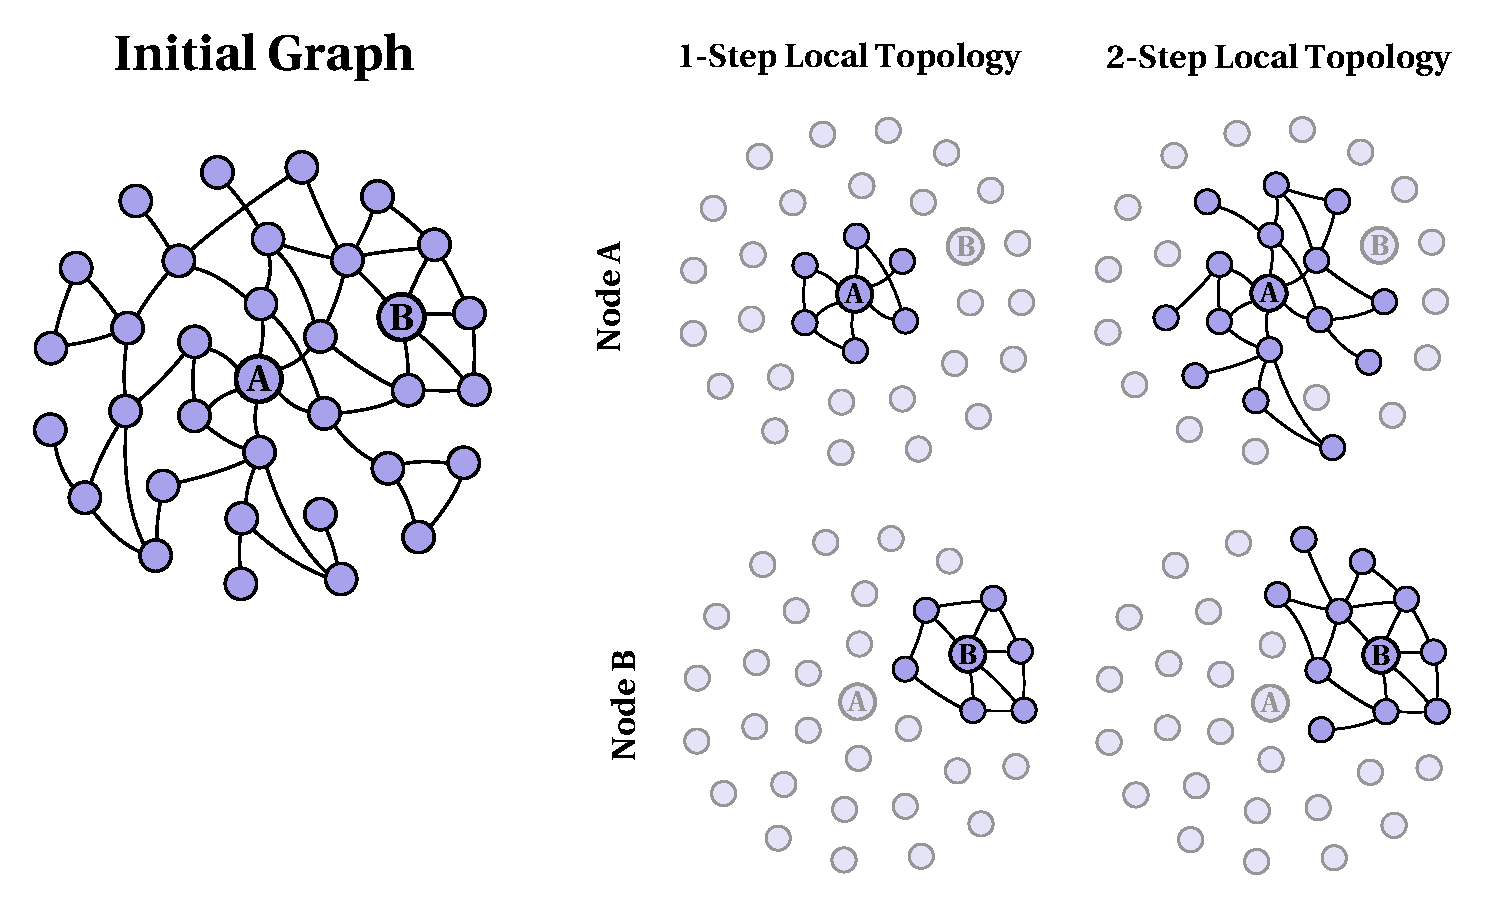
\includegraphics[width=0.8\textwidth]{fig/fig1.pdf}
  \caption{Illustration of the 1-step and 2-step local topologies for two nodes in an undirected graph.}
  \label{fig:localTopology}
\end{figure*}

\subsection{Fixed Node Edit Distance (FNED)}
Our first step towards embedding involves defining a distance between the local topologies around nodes; we describe how these distances are used for the Euclidean embedding in Section~\ref{sec:algos}. The concept of edit distance has been shown to provide an intuitive way to represent distances between abstract structures \cite{riesen2009approximate,reis2004automatic,gao2010survey}. We aim to define an edit distance between the local topologies around nodes in a graph. We call this the Fixed Node Edit Distance (FNED), and define it to be the minimum number of edge insertions or deletions to transform the local topology around one node into the local topology around another node.

An equivalent definition of the FNED, which we refer to as the mapping-overlap formulation, allows for easier computation. Intuitively, for a given mapping between the nodes of a pair of local topologies, we can find the number of edges that ``do not overlap" (i.e. given the mapping, the number of node-pairs that are adjacent in one of the two local topologies but not adjacent in the other). The mapping that yields the minimum number of non-overlapping edges is equivalent to the FNED defined in terms of minimal edit distance.

Formally, for a graph $G = \{V,E\}$, let $\Omega_{V}$ be the set of bijections from $V$ to itself (i.e. the set of permutations of $V$). Additionally, let $\Omega_{V, a\rightarrow b}$ be $\Omega_{V}$ restricted to bijections where node $a\in V$ is mapped to node $b\in V$. For all vertices $a,b \in V$, we define the FNED between $a$ and $b$ (given the two $k$-step local topologies $T_{k}(a)$ and $T_{k}(b)$), to be
\begin{equation}
\text{FNED}_{k}(a,b) = \text{min} \big|_{m \in \Omega_{V, a\rightarrow b}} d(T_{k}(a), T_{k}(b), m)
\end{equation}
where
\begin{equation}
\begin{split}
d(T_{k}(a), & T_{k}(b), m) = \\ 
& \sum_{i=1}^{n} \sum_{j=i}^{n} \Big[ A_{T_{k}(a)}(m(i),m(j)) \oplus A_{T_{k}(b)}(i,j)  \Big]
\end{split}
\end{equation}
where $A_{G}$ denotes the adjacency matrix of graph G. Given adjacency matrices $A_{G_{1}}$ and $A_{G_{2}}$, both of size $n \times n$, we define the XOR operator $\oplus$ to be
\begin{equation}
A_{G_{1}}(i_{1},j_{1}) \oplus A_{G_{2}}(i_{2},j_{2}) = 
\begin{cases}
1 \text{ if } A_{G_{1}}(i_{1},j_{1}) = A_{G_{2}}(i_{2},j_{2}) \\ 
0 \text{ otherwise}
\end{cases}
\end{equation}
We illustrate the two definitions of the FNED and show an example of the distance between two nodes in Figure~\ref{fig:fnedFigure}. In this figure, for the nodes $A$ and $B$ given in Figure~\ref{fig:localTopology}, we depict the FNED as a minimal sequence of edits, and as an mapping that yields the minimum number of non-overlapping edges.

This paper is focuses only on undirected graphs, through it can be extended to directed and other labelled graphs by modifying the allowable edge edit operations.

\begin{figure*}[h!tbp]
  \centering               
  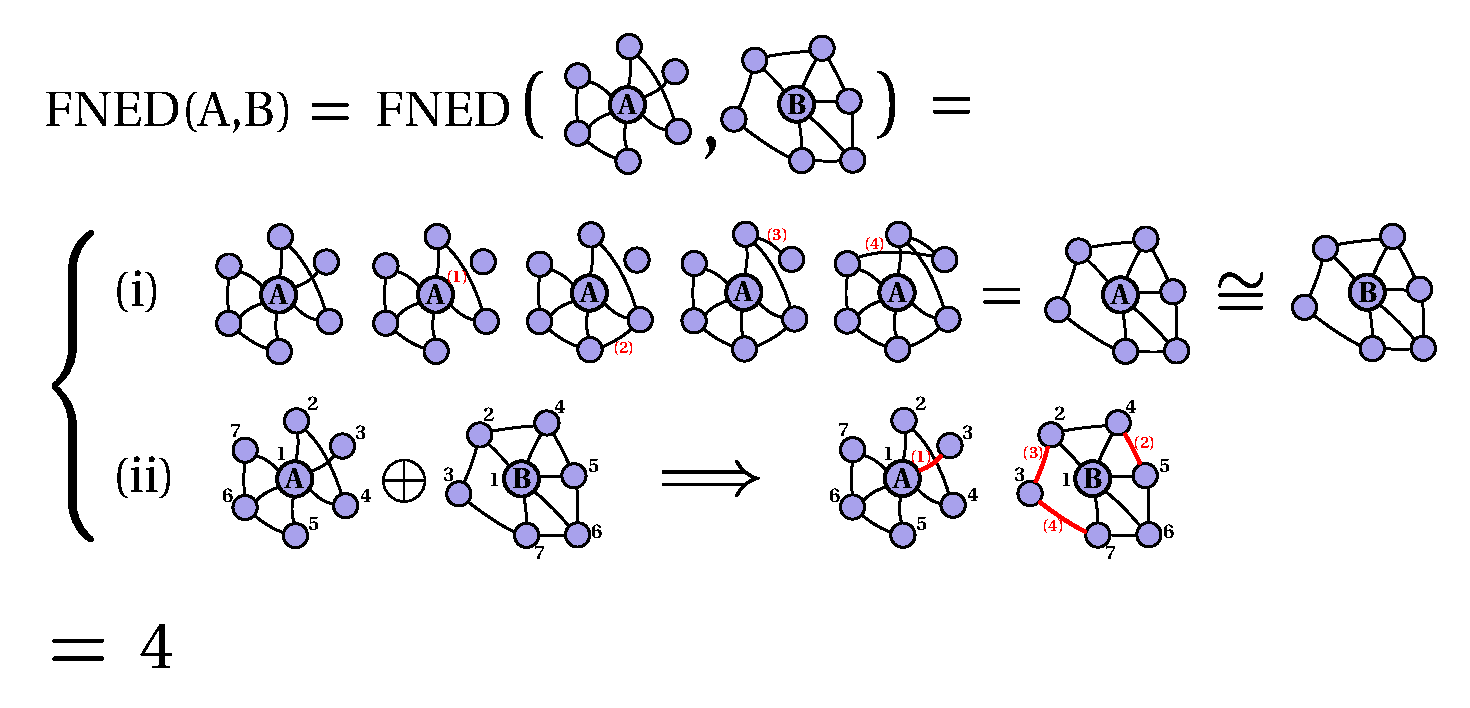
\includegraphics[width=0.8\textwidth]{fig/fig2.pdf}
  \caption{Illustration of the FNED between two local topologies. (i) shows the FNED viewed as a minimal sequence of edge edits, while (ii) shows an equivalent definition of the FNED (the mapping-overlap formulation) as a minimal collection of edges that ``do not overlap'' (colored red) for a given mapping.}
  \label{fig:fnedFigure}
\end{figure*}


\section{Algorithms for Embedding}
\label{sec:algos}
The algorithms in this section describe the process of embedding the nodes of a graph in Euclidean space based on their local topologies.

\subsection{Overview for Embedding Nodes}
Algorithm~\ref{alg:overviewEmbedding} gives an overview of the process of embedding in Euclidean space each node in a graph, based on its local topology.

\begin{algorithm}[h!tbp]
\caption{Node Embedding via Local Topologies}
\label{alg:overviewEmbedding}
\begin{algorithmic}[1]
\STATE \textbf{Input:} \\(i) An undirected graph, $G = \{V,E\}$.\\(ii) A local topology step size, $k$.\\(iii) A set of basis nodes, $B \subset V$.
\FOR{each $v \in V$}
\FOR{each $b \in B$}
\STATE Set $\text{Embedding}(v,b) = \text{FNED}_{k}(v,b)$
\ENDFOR
\ENDFOR
\STATE \textbf{Output:} Embedding, the feature matrix where each row is a node, and the set of columns represents the embedding $\in \mathbb{R}^{B}$.
\end{algorithmic}
\end{algorithm}

The embedding into Euclidean space is wholly dependent upon computation of the FNED between the local topologies of the nodes. The algorithms in the following sections provide different methods for computing the FNED, given certain graph types.


\subsection{Deterministic FNED for Trees}

In Algorithm~\ref{alg:trueFnedTrees} we give a polynomial time algorithm for computing the FNED between nodes in a tree for 2-step local topologies. We will give approximate algorithms for computing the FNED between nodes in an arbitrary graph in Section~\ref{sec:approxFned}, as the FNED is, in general, not possible to compute exactly in polynomial time. Algorithm~\ref{alg:trueFnedTrees} can also be used as a basis for approximate FNED computation in arbitrary graphs for $2$-step local topologies.
\begin{algorithm}[h!tbp]
\caption{Deterministic FNED for Trees}
\label{alg:trueFnedTrees}
\begin{algorithmic}[1]
\STATE \textbf{Input:} \\(i) An undirected graph, $G = \{V,E\}$ without loops.\\(ii) Two nodes: $A, B \in V$.
\STATE{Compute $T_{2}(A)$ and $T_{2}(B)$, the local topologies of $A$ and $B$.}
\STATE{$N = \text{max}(|T_{2}(A)|, |T_{2}(B)|)$}
\STATE{Add $N-\text{min}(|T_{2}(A)|, |T_{2}(B)|)$ disconnected ``virtual nodes'' to the local topology with less nodes.}
\FOR{each $a \in T_{2}(A)$ adjacent to $A$}
\FOR{each $b \in T_{2}(B)$ adjacent to $B$}
\STATE Find $n_{a} = \# \{ a' | a' \text{ adjacent to } a \text{ and } a' \neq A \}$
\STATE Find $n_{b} = \# \{ b' | b' \text{ adjacent to } b \text{ and } b' \neq B \}$
\STATE Set $\text{CostMatrix}(a,b) = | n_{a} - n_{b} |$
\ENDFOR
\ENDFOR
\STATE $\text{OptMap}=\text{HungarianAlgorithm}(\text{CostMatrix})$
\STATE $\text{FNED}_{k}(A,B) = \sum_{i=1}^{|T_{2}(A)|} \text{XOR}(i,\text{OptMap}(i))$
\STATE \textbf{Output:} $\text{FNED}_{k}(A,B)$, the fixed node edit distance between $A$ and $B$ for $k$-step local topologies.
\STATE Note 1: HungarianAlgorithm() returns an optimal mapping between nodes adjacent to $A$ and nodes adjacent to $B$ given CostMatrix.
\STATE Note 2: XOR(i,j) returns $|n_{i} - n_{j}|$ (defined on lines 7 and 8) for $i \in T_{2}(A)$ and $j \in T_{2}(B)$.
\end{algorithmic}
\end{algorithm}

% What is the following algorithm for? how it is different than above algo?
% ----------------------------------------------------------------
% \begin{algorithm}[!]
% \caption{Deterministic True FNED for Trees}
% \label{alg:trueFnedTrees}   % haven't gotten this label to work for some reason
% \begin{algorithmic}[1]
% \STATE \textbf{Input:} \\(i) An undirected graph, $G = \{V,E\}$ without loops.\\(ii) A local topology step size, $k$.\\(iii) Two nodes: $A, B \in V$.
% \STATE{steps $= 0$}
% \FOR{each $a \in V$ adjacent to $A$}
% \FOR{each $b \in V$ adjacent to $B$}
% \IF{steps $= k$}
% \STATE Set $\text{CostMatrix}(a,b) = \text{difference}$
% \ELSE
% \STATE Set $k = k+1$ 
% \STATE Compute CostMatrix for all adjacent nodes.
% \STATE Compute OptimalMap with HungarianAlgorithm.
% \STATE Compute XOR edge distance for given map.
% \ENDIF
% \ENDFOR
% \ENDFOR
% \STATE $\text{OptimalMap}=\text{HungarianAlgorithm}(\text{CostMatrix})$
% \STATE Compute XOR edge distance for given map.
% \STATE \textbf{Output:} $\text{FNED}_{k}(A,B)$, the fixed node edit distance between A and B for $k$-step local topologies.
% \end{algorithmic}
% \end{algorithm}


\subsection{Approximate FNED for Arbitrary Graphs}
\label{sec:approxFned}

Finding an optimal graph matching is not possible in polynomial time for arbitrary graphs. In this section we provide a Markov Chain Monte Carlo (MCMC)-based algorithm to search the combinatorial space of mappings between the nodes of two local topologies. The algorithm follows a directed random walk through the space of permutations of nodes in a local topology in order to minimize the FNED (adhering to the mapping-overlap formulation of the FNED).

% \subsubsection{Tree Based Heuristic}

\subsubsection{MCMC for Computing the FNED}
Here, we formulate computation of the FNED between nodes as a stochastic combinatorial optimization problem. In Algorithm~\ref{alg:fnedMcmc} we describe an MCMC algorithm similar to Metropolis-Hastings for sampling the FNED between two nodes in an arbitrary graph.

\begin{algorithm}[h!tbp]
\caption{MCMC for FNED in Arbitrary Graphs}
\label{alg:fnedMcmc}
\begin{algorithmic}[1]
\STATE \textbf{Input:} \\(i) An undirected graph, $G = \{V,E\}$.\\(ii) A local topology step size, $k$.\\(iii) Two nodes: $A, B \in V$\\(iv) Maximum sampling iteration, NumIter.
\STATE{Compute $T_{k}(A)$ and $T_{k}(B)$, the $k$-step local topologies of $A$ and $B$.}
\STATE{$N = \text{max}(|T_{k}(A)|, |T_{k}(B)|)$}
\STATE{Add $N-\text{min}(|T_{k}(A)|, |T_{k}(B)|)$ disconnected (degree 0) nodes to the local topology with fewer nodes.}
\STATE{Initialize a mapping $m$ between nodes in $T_{k}(A)$ and nodes in $T_{k}(B)$}
\FOR{$i=1:\text{NumIter}$}
\STATE{$m' = m$}
\STATE{Randomly choose 3 nodes $\in T_{k}(a)$, and randomly permute their mapping in $m'$}
\IF{$d(T_{k}(a), T_{k}(b), m') < d(T_{k}(a), T_{k}(b), m)$}
\STATE{Set $m = m'$}
\STATE{Record $d(T_{k}(a), T_{k}(b), m)$}
\ELSE
\IF{rand() $ < \frac{d(T_{k}(a), T_{k}(b), m)}{d(T_{k}(a), T_{k}(b), m')}$}
\STATE{Set $m = m'$}
\STATE{Record $d(T_{k}(a), T_{k}(b), m)$}
\ENDIF
\ENDIF
\ENDFOR
\STATE $\text{FNED}_{k}(A,B)$ = the minimum $d(T_{k}(a), T_{k}(b), m)$ over $m$ through all iterations.
\STATE \textbf{Output:} $\text{FNED}_{k}(A,B)$, the fixed node edit distance between $A$ and $B$ for $k$-step local topologies.
\STATE{Note 1: $d(T_{k}(a), T_{k}(b), m)$ is defined in Section~\ref{sec:defs}}.
\STATE{Note 2: rand() returns a uniformly distributed random number $\in (0,1)$}
\end{algorithmic}
\end{algorithm}


\section{Experiments}
\label{sec:exp}

% \subsection{Exploring the Embeddings of Nodes in Random Trees}
% This experiment illustrates the embeddings of nodes in synthetically generated random tree graphs. 


\subsection{Assessment of Role Discovery on Synthetic Graphs}
We'd like to asses the performance of this method on synthetic data containing nodes with known roles (i.e. nodes with pre-specified types of local topologies), in order to judge whether the method is able to accurately find groups of nodes with similar topological structures in a graph. To carry out this synthetic experiment, we defined a simple model for roles in a network consisting of a Gaussian mixture over the node degrees and a Gaussian mixture over the number of edges 


\subsection{Demonstration of Method on Small Social Networks}
We apply our method to two well studied social network datasets. The first shows friendships among members of a karate club at a US university \cite{zachary1977information}, and the second consists of associations among a collection of dolphins \cite{bottleNoseDolphinPeople}.
\begin{figure*}[h!tbp]
  \centering               
  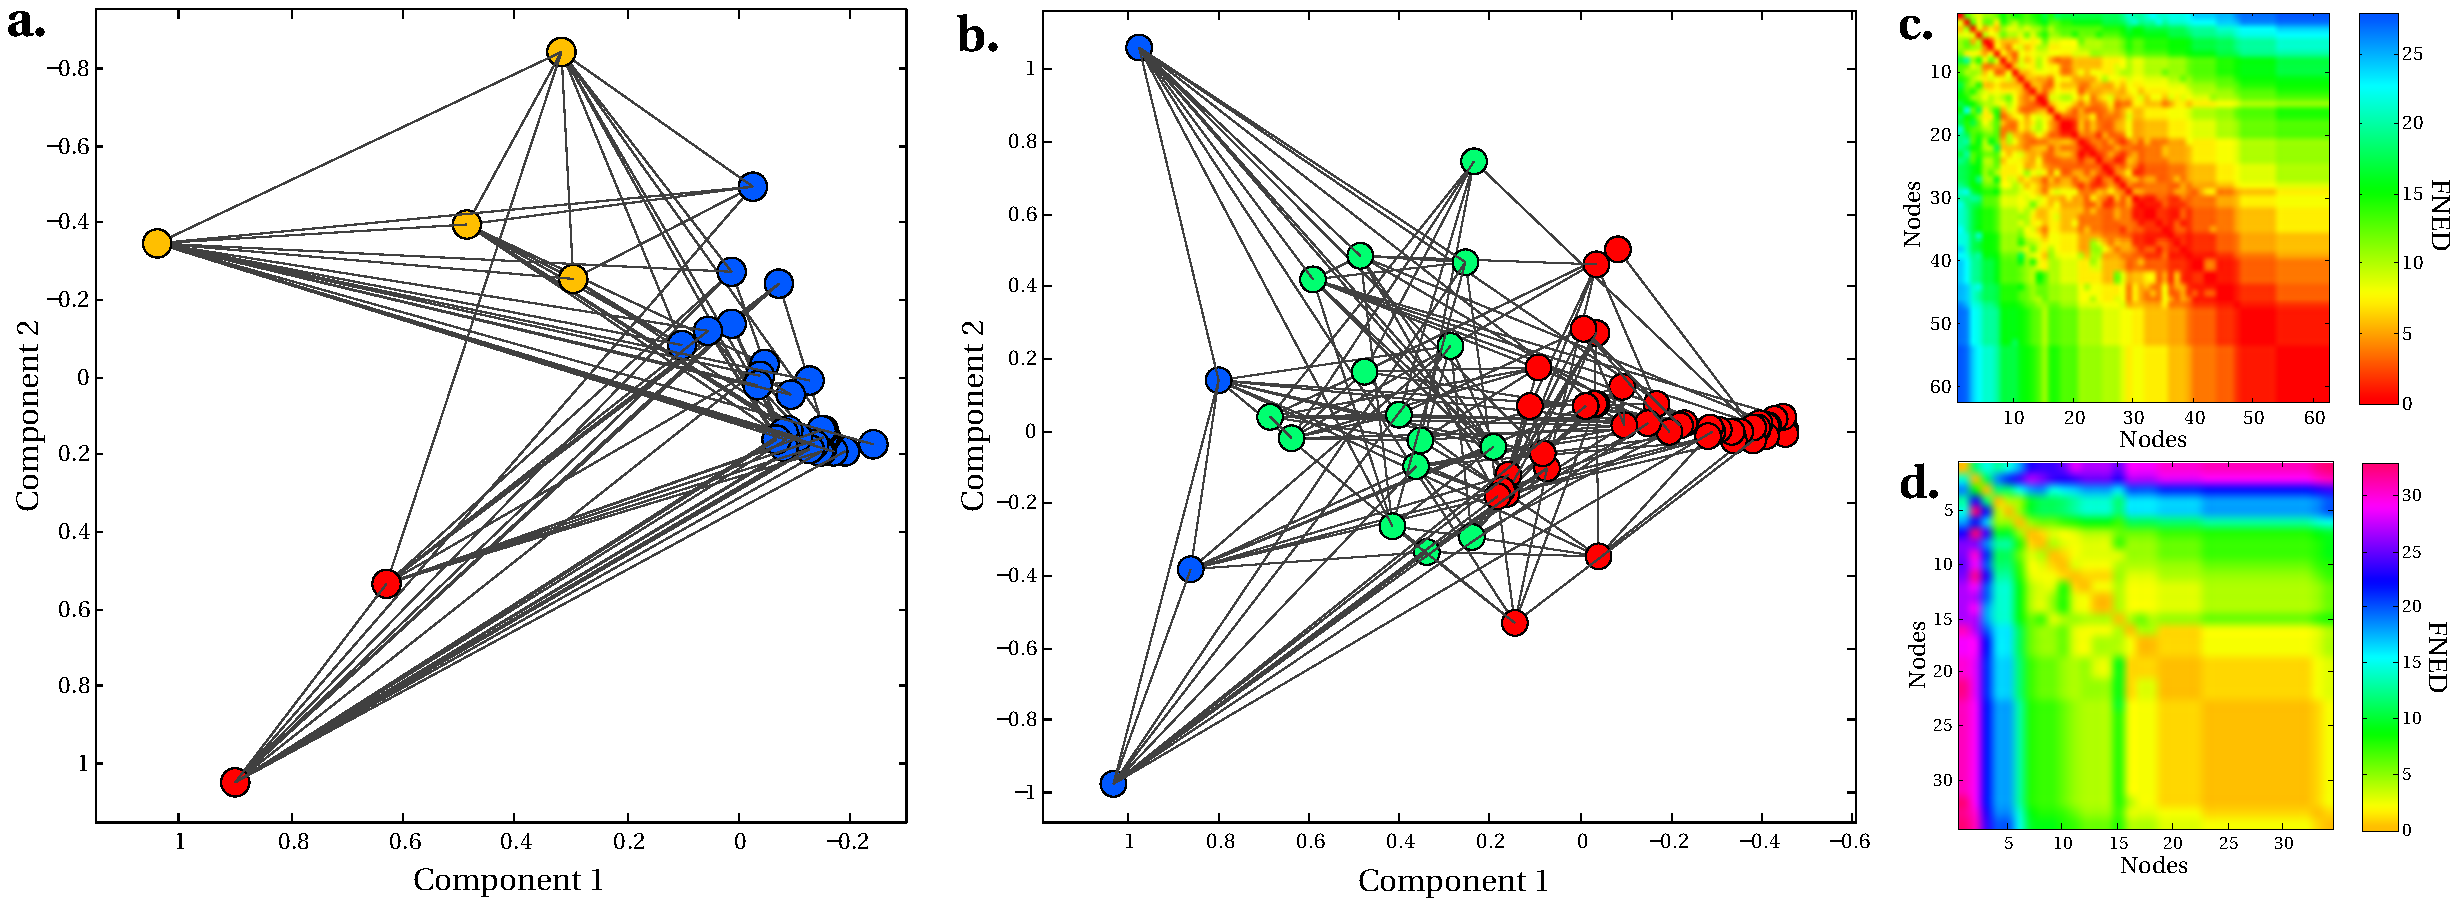
\includegraphics[width=1\textwidth]{fig/fig3.pdf}
  \caption{Results of embedding and role-clustering for two social networks. (a) The first two MDS components of each embedded node in the karate club social network dataset and (b) dolphin social network dataset. The network edges are drawn and the nodes are colored based on clustering the embedded points. (c) A heatmap encoding the Euclidean embedding for nodes in the dolphin social network dataset and (d) karate club social network dataset.}
  \label{fig:smallSocialNetwork}
\end{figure*}

Embedding was performed using the MCMC algorithm to compute the FNED between 1-step local topologies for both datasets. After embedding, the $k$-means algorithm was carried out to cluster the nodes into groups with similar local topologies. The $k$-means algorithm was initialized at ten clusters, and converged to three clusters in both datasets. The entities in both networks were partitioned based on their social patterns, with the largest cluster containing a collection of low-degree nodes, and the other two clusters splitting the high-degree nodes into groups based on the connectivity between their adjacent nodes.

To visualize the embedding, multidimensional scaling (MDS) was applied to reduce the dimension of embedded nodes. Figure~\ref{fig:smallSocialNetwork} plots the first two MDS components, with marker color denoting the clustering results. In both plots, the node degree tends to decrease when moving from left to right across the $x$-axis. Nodes with a low degree tend to cluster together and those with a high degree tend to spread further apart, due to the potential for increased topological complexity around higher-degree nodes. Figure~\ref{fig:smallSocialNetwork} also displays the embedding for all nodes in each graph as a heatmap. Heatmaps are useful for visualizing the embedded nodes (the $i^{th}$ row/column represents the $i^{th}$ node's vector embedding) and identifying groups of points with similar local topologies.


\subsection{The Topology Among Teams in College Football Conferences}
The datset in this experiment consists of a network of college football teams \cite{newman2006finding}. Edges connect pairs of teams if they are scheduled to play each other. This dataset provides a label for each team representing its conference (out of 12 possible conferences). 

In this experiment, instead of clustering the embedded points, we color each according to its conference association. We aim to assess whether teams in a given conference have similar local topologies (we'd expect this to be the case, as there exist per-conference policies regarding the number of games played against in-conference and out-of-conference opponents).

\begin{figure*}[h!tbp]
  \centering               
  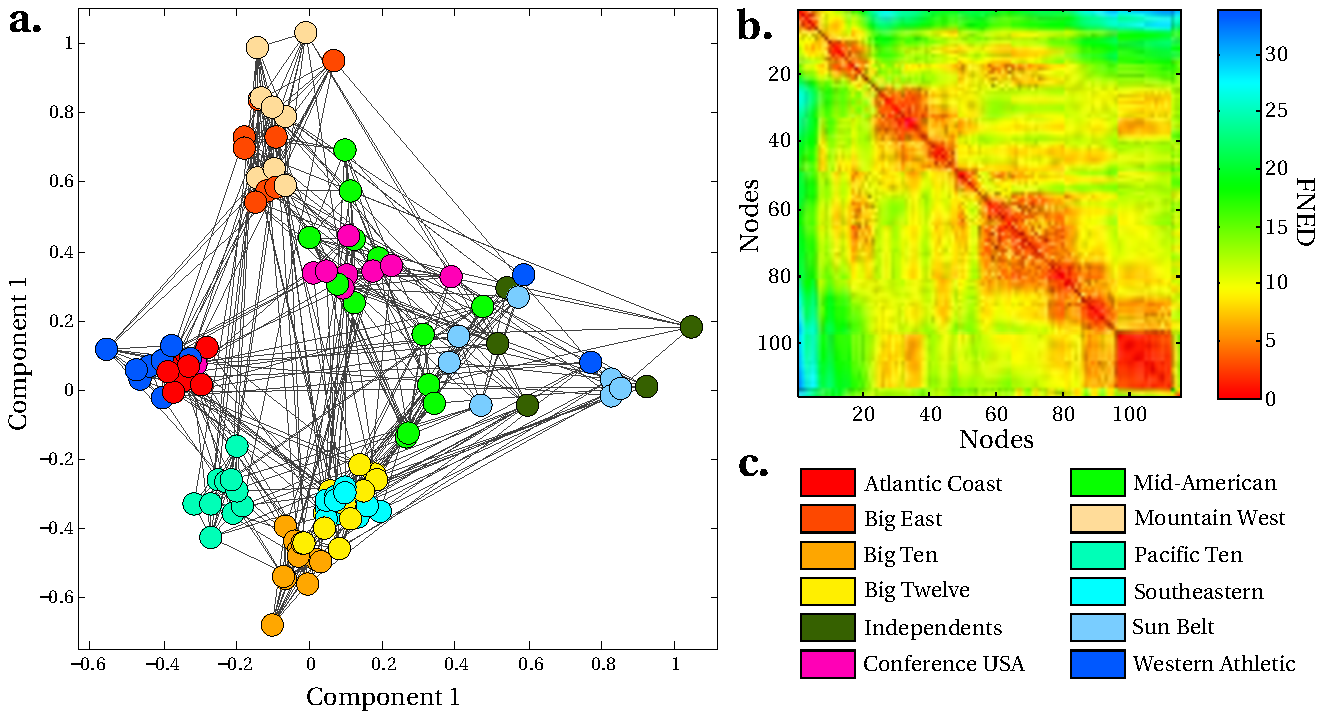
\includegraphics[width=1\textwidth]{fig/fig4.pdf}
  \caption{A network of college football team matchups during a given season is shown. Markers are colored based on the league (out of 12) in which the associated team resides. Teams belonging to the same league tend to be embedded similarly, as do teams from similar geographic locations.}
  \label{fig:footballTeams}
\end{figure*}

Embedding was performed using the MCMC algorithm to compute the FNED between 1-step local topologies. Figure~\ref{fig:footballTeams} shows the first two MDS components of the Euclidean embedding. This figure also shows the correspondence between each node and its conference label. We find that the embedding often places football teams from the same conference at similar points in space. This is reflected in the heatmap displaying the embedding of all nodes, where we see clear clusters along the diagonal. Figure~\ref{fig:footballTeams} allows us to see which conferences have teams with very similar (e.g. Pacific Ten) or more varied (e.g. Mid-American) local topologies, which conferences are similar to others in terms of the local topologies of their teams, and in a couple cases, which teams have a local topology distinct from the others in their conference. 


\subsection{Role Discovery in Larger Networks and Comparisons with Node Degree}
In this experiment, we hope to demonstrate the ability of our method to discover groups of nodes with similar roles in larger networks, and explicitely compare our descriptor of local topology around a node with the node's degree. We apply our method two two networks: a neural network of the nematode C. Elegans \cite{pujol2001reverse,watts1998collective}, and a coauthorship network for network scientists \cite{newman2006finding}.


The dataset in this experiment consists of the 60 most common nouns and adjectives in Charles Dickens' David Copperfield \cite{newman2006finding}. Edges are assigned between words if they appear adjacent to each other at any point in the text.

In this experiment, we hope to show that the embedding method described in this paper yields features that could be used to benefit a supervised machine learning problem; if so, Euclidean local topology features could be added to the features of datasets that are equipped with information about relationships between data elements. In particular, we hope to see some sort of differentiation between the embedding of adjectives and the embedding of the nouns in this dataset.

\begin{figure*}[h!tbp]
  \centering               
  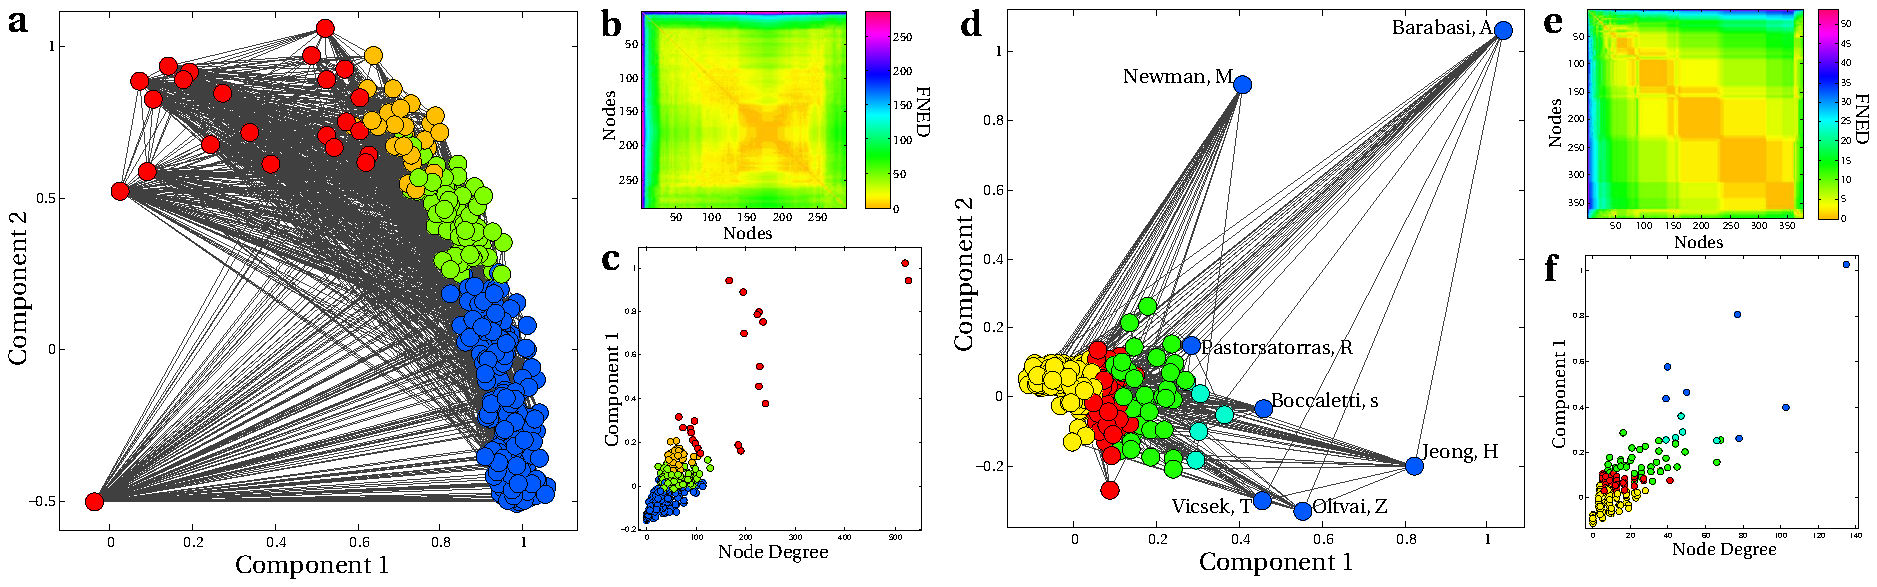
\includegraphics[width=1\textwidth]{fig/fig5.pdf}
  \caption{The 60 most common adjectives and nouns in Dickens' David Copperfield. Red markers denote adjectives and blue markers denote nouns. Words of different types tend to be embedded in different positions in space.}
  \label{fig:dickensCopperfield}
\end{figure*}

Embedding was performed using the MCMC algorithm to compute the FNED between 1-step local topologies. Figure~\ref{fig:dickensCopperfield} plots the first two dimensions (and first three dimensions on the right) of the embedding feature vectors. A few of the words, along with the graph edges, are shown in the two plots. Adjectives are colored red and nouns are colored blue. From this embedding, we can see that the adjectives and nouns are slightly differentiated in the embedding space. Additionally, a group of adjectives are isolated from the rest of the words.


\section{Conclusion}
\label{sec:conclusion}

We have introduced a method for representing the local topology around a node in Euclidean space by defining the $k$-step local topology and fixed node edit distance between nodes. Additionally, we have provided two algorithms for computing the FNED between nodes of different types of graphs, and have demonstrated this embedding on three publically available datsets. Our demonstrations have shown that the Euclidean local topology features can be used alone to perform graph clustering of nodes into groups with similar local topologies, or can provide additional features for datasets equipped with relationships between their elements, in order to benefit a supervised learning task. 


\begin{small}
\bibliographystyle{plainnat}
\bibliography{paper_refs} 
\end{small}

\end{document}


% \begin{figure}[h]
%   \centering             
%   \subfloat[]{\includegraphics[width=0.32\textwidth]{../img/kmeans_2.pdf}}
%   \hspace{1mm}
%   \subfloat[]{\includegraphics[width=0.32\textwidth]{../img/kmeans_3.pdf}}
%   \hspace{1mm}
%   \subfloat[]{\includegraphics[width=0.32\textwidth]{../img/kmeans_4.pdf}}
%   \caption{K-means clustering results on the 5 frame sequences of cell speeds extracted from time lapse microscopy video data. The mean speed (over all sequences) is subtracted from each value of each sequence for detrending. Speed in relative units is displayed on the y axis. The color of each sequence denotes its cluster assignment. Results are shown for $K=2$ (a), $K=3$ (b), and $K=4$ (c).}
%   \label{fig:kmeans}
% \end{figure}


% \begin{figure}[h]
%   \centering             
%   \subfloat[]{\includegraphics[width=0.28\textwidth]{../img/control.pdf}}
%   \hspace{1mm}
%   \subfloat[]{\includegraphics[width=0.28\textwidth]{../img/raromix.pdf}}
%   \hspace{1mm}
%   \subfloat[]{\includegraphics[width=0.28\textwidth]{../img/well6.pdf}}
%   \caption{Three example frames from the benchmark cell video datasets used in experiments one (a), two (b), and three (c). }
%   \label{fig:cell_imgs}
% \end{figure}
